\documentclass[a4paper,13pt]{report}

\usepackage[top=2.5cm,bottom=2.5cm,left=3cm,right=2cm]{geometry}
\usepackage{graphicx}
\usepackage[english]{babel}
\usepackage[utf8]{inputenc}
\usepackage[T1]{fontenc}
\usepackage{ragged2e}
\usepackage{hyphenat}
\usepackage{lmodern}
\usepackage{fancyhdr}
\usepackage[toc,page]{appendix}
\usepackage{tabularx}
\usepackage{float}
\usepackage{amsmath}
\usepackage{indentfirst}
\usepackage[table]{xcolor}
\usepackage{array,multirow} 
\usepackage{varwidth}

\setcounter{secnumdepth}{4}

\begin{document}
    \centering
    \LARGE{\textsc{VIETNAM AVIATION ACADEMY}}\\
    \vspace{3mm}
    \normalsize{Department of Telecommunication - Electronics Engineering Technology} \\
    \vspace{3mm}
    \large{LOCATION IN HO CHI MINH CITY} \\
    \vspace{3mm}
    
\includegraphics[scale=0.3]{logo.jpg} \\
    \vspace{3mm}
    \normalsize{PROJECT REPORT: } \\ 
    \vspace{15mm}
    \huge{\textbf{"Radar detector module using Arduino"}} \\
    \vspace{20mm}
    \normalsize{Written by} \\
    \vspace{3mm}
    \large{\textbf{\textit{Nguyen Van Anh Tuan}}} \\
    \vspace{3mm}
    \textbf{{\large{\textit{Roll.No.1753020018}}}} \\
    \vspace{15mm}
    \large{Under the guidance of} \\ 
    \vspace{10mm}
    \centerline{\textbf{\large{Master.Cao Xuan Kim Anh}}}
    
    %Lines down here is set header and footer
    \pagestyle{fancy}
    \fancyhf{}
    \rhead{Radar detector module}
    \lhead{Anh Tuan}
    \cfoot{\today}
    \renewcommand{\headrulewidth}{2pt}
    \renewcommand{\footrulewidth}{1pt}

    % \setlength\parindent{24pt} is indentation.
    \newpage
    \centering
    \centerline{\textbf{\huge{PREAMBLE}}}
    \vspace{10mm}
    \begin{flushleft}
        Radar is an object detection system. It uses Microwaves to determine the range, 
        altitude, or speed of objects. The radar can transmit radio waves or microwaves 
        which bounce off any object in their path. So, we can easily determine any object 
        in the radar range. Arduino is a single-board microcontroller to make electronics 
        more discipline. The radar system has different performance specifications and also 
        it comes in a verity of size.
    \end{flushleft}
    \begin{flushright}
        \textbf{Auth. Nguyen Van Anh Tuan}
    \end{flushright}
    \thispagestyle{plain}

    \newpage
    \tableofcontents

    \chapter{Introduction}
    \renewcommand{\headrulewidth}{0.5pt}
    \renewcommand{\footrulewidth}{0.5pt}
    \thispagestyle{fancy}
    \fancyhf{}
    \fancyhead[L]{\textbf{CHAPTER 1}}
    \fancyhead[R]{\textbf{Radar Detector Module}}
    \raggedright
    \fancyfoot[R]{Page \thepage}
    \section{PRELIMINARY INTRODUCTION}
    \subsection{The reason why to choose project}
        With the passion for aviation as well as passion for technology and equipment realted to 
        it, i decided to choose an aviation-related project in this project. Fortunately, my project 
        this time is on topic of embedded programming. So, i choose project named "PSR radar 
        detector module using Arduino". In this project, i will rely 
        on the PSR radar to make a small scale PSR radar detector model. So, to get 
        started in this project, we need to know what PSR radar is and how it works. \\
    \vspace{5mm}
        Recognize the continuous development of aviation technology. I want to add my own 
        knowledge about how a radar system works and a bit of creative idea for this device 
        that came along during i make this project. And that's why i choose this project for myself. \\
    \vspace{5mm}
    \textbf{Block diagram}
    \begin{figure}[ht]
        \centering
        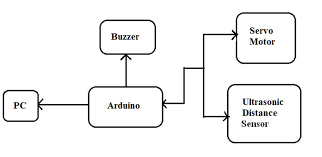
\includegraphics[scale=0.7]{block_diagram.png}
        \caption{\label{fig:pic}Block diagram for radar model}
    \end{figure}
    \linebreak
    \par You may ask how the processing application works here. It's very simple, the 
    Ultrasonic sensor collects the object information with the help of Arduino and passes 
    it to processing application, there is a simple Graphics application implemented which 
    mimic a radar screen.
    \subsection{Target Research}
        The short term goal of this topic is with the desire to learn and supplement the 
        knowledge that in the course of research. With the long term goal, i want to perform 
        the topic in the best way i can. As well as improve the errors of myselft. And also, 
        i want to additional the knowledge i haven't learned at my school.
    \subsection{Object and position research}
    \vspace{3mm}
        \begin{itemize}
            \item \textbf{Object Research:} The object that i study is the sensor system 
        installed on the air traffic control station or installed on robots that detect 
        objects and avoid them.
            \item \textbf{Position Research:} My reserach is based on the application of radar 
        to detect missing vehicles or to apply air traffic control as call as "Primary Surveillance Radar".
        \end{itemize} 
    \subsection{Method of research}
        \begin{itemize}
            \item \textbf{Observation Method:} By observing directly at air traffic control 
        and also via movies or aviation videos on internet.
            \item \textbf{Method of analysis:} Looking for some similar projects that have 
        been made available online, from the detailed data of those projects, i draw some 
        methods and experience for my project. Avoid mistakes in my project.
        \end{itemize}
    \subsection{Structure Project}
        My article is divided into three main sessions, summarized as follow: 
        \begin{itemize}
            \item In the first chapter, i will focus on brief introduce my project, presenting 
        some of the research content on the topic of the method of conducting research that 
        gives practical results during the project research process.
            \item The second chapter, is an content and result of project. Besides is a block diagram 
        how the project working and circuit diagram of my project.
            \item Chapter three is the chapter where i introduce and explain the code i used in this project.
            \item Chapter four is the chapter for giving conclusions and recommendations about my project.
            \item And the final chapter is the final section where i list the sources of reference i have 
        used in this project.
        \end{itemize}
    \newpage
    \section{BASIC THEORY}
    \subsection{Theory about the radar}
        At first, before we learn about how this project works, let's take a quick look at the 
        definition of radar. Now we can see objects in the world around us because light(usually 
        from the Sun) reflects off them into your eyes. If you want to walk at night, you can shine 
        a torch in front to see where are you going. \\
        \vspace{1mm}
        \par Radar works in much the same way. The word "Radar" stands for \textbf{RA}dio \textbf{D}etection 
        \textbf{A}nd \textbf{R}anging, and that gives a pretty big clue as to what it does and how 
        it works. Imagine an airplane flying at night through thick fog. The pilot can't see where 
        are they going, so they use the radar to help them. \\
        \vspace{1mm}
        \par An airplane's radar is a bit like a torch that uses radio waves instead of light. The 
        plane transmits and intermittent radar beam (so it sends a signal only part of the time) 
        and for the rest of the time.
    \subsection{Some research related to the project}
        Some research ideas related to my project:
        \begin{itemize}
            \item The function contained in some robots, helps robots scan the terrain 
        and detect objects to avoid.
            \item Radar in the Air traffic control tower named "Primary Surveillance Radar"
        \end{itemize}
    \subsection{Theory concepts related to research issues}
        \begin{itemize}
            \item \textbf{PSR(Primary Surveillance Radar)}: A Surveillance radar system which
        uses reflected radio signals.
            \item \textbf{US(Ultrasonic Sensor)}: As the name indicates, ultrasonic sensors 
        measure distance by using ultrasonic waves.
            \item \textbf{PWM(Pulse-Width Modulation)}: is a method of reducing the average 
        power delivered by an electrical signal, by effectively chopping it up into discrete parts.
            \item \textbf{RAM(Random-Access Memory)}: is a form of computer memory that can be 
        read and changed in any order, typically used to store working data and machine code.
            \item \textbf{CPU(Central Processing Unit)}: also called a central processor or main 
        processor, is the electronic circuitry within a computer that executes instruction that 
        make up a computer program.
        \end{itemize}
    \subsection{Components Required}
        \begin{enumerate}
            \item For power:
            \setlength{\parindent}{4em}
            Micro USB-B
            \item For radar model:
            \begin{enumerate}
                \item Arduino UNO
                \item Servo motor
                \item Ultrasonic Sensor HRF-04
                \item Buzzer
                \item LCD 16x02
                \item LED (green, red)
                \item Test board
            \end{enumerate}
        \end{enumerate}
    \newpage
    \subsection{Component Description}
        \vspace{3mm}
        \subsubsection{\Large{Arduino Uno}}
            \vspace{3mm}
            \begin{enumerate}
                \item \textbf{Introduction about Arduino UNO}
                \linebreak
                \par Arduino UNO is a microcontroller board developed by Arduino.cc which is open-source 
                electronics platform mainly based on AVR microcontroller ATMega328. \\
                \vspace{3mm}
                \par First Arduino projcet was started in Interaction Design Institute 
                Ivrea in 2003 by David Cuartielles and Massimo Banzi with the intention of 
                providing a cheap and flexible way to students and professional for controlling 
                a number of devices in the real world. \\
                \vspace{3mm}
                \par The current version of Arduino UNO comes with USB interface, 6 analog 
                input pins, 14 I/O(input/output) digital ports that are used to connect with 
                external electronic circuit. Out of 14 I/O ports, 6 pins can be used for PWM output.\\
                \vspace{3mm}
                \par It allows the designers to control and sense the external electronic devices in 
                the real world. \\
                \vspace{3mm}
                \par Apart from USB, battery or AC to DC adopter can also be used to power the board. \\
                \vspace{3mm}
                \par There are many versions of Uno board available. However, Arduino Uno V3 and Arduino 
                Uno are the most official versions that come with ATMega328 8-bit AVR Atmel microcontroller 
                where RAM memory is 32KB.
                \begin{figure}[ht]
                    \centering
                    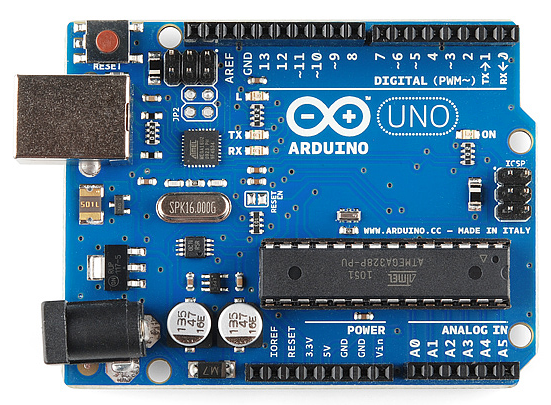
\includegraphics[width=0.5\linewidth]{Uno.png}
                    \caption{\label{fig:pic}Arduino Uno board}
                \end{figure}
                \item \textbf{Features}
                    \linebreak
                    \begin{figure}[ht]
                        \centering
                        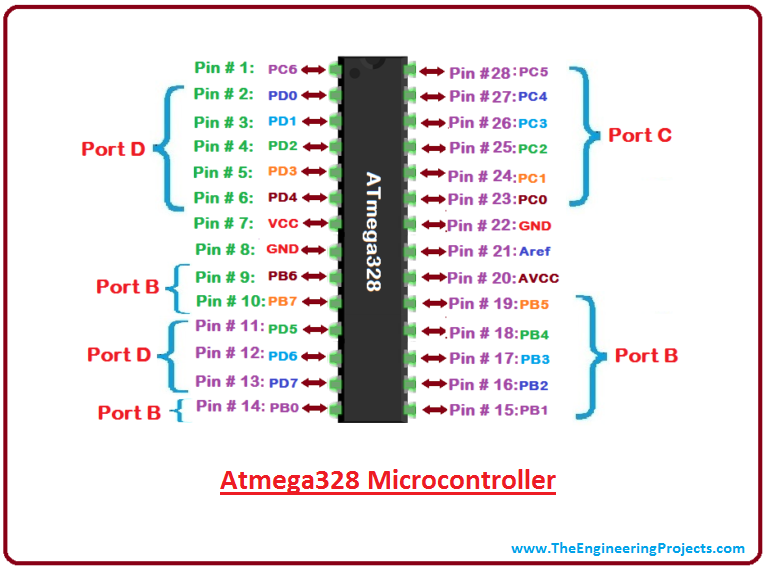
\includegraphics[width=0.6\linewidth]{atmega.png}
                        \caption{\label{fig:pic}ATMega328 Microcontroller}
                    \end{figure}
                \begin{itemize}
                    \item Comes with USB interface.
                    \item USB port is added on the board to develop serial communication with the computer
                    \item ATMega328 microcontroller is placed on the board that comes with a number of 
                features like timers, counters, interrupts, PWM, CPU, I/O pins and based on a 16MHz clock 
                that helps in producing more frequency and number of instruction per cycle.
                    \item It's an open-source platform where anyone can modify and optimize the 
                board based on the number of instructions and task they want to achieve.
                    \item Come with a built-in regulation feature which keeps the voltage under control 
                when the device is connected to the external device.
                    \item There are 14 pins I/O digital and 6 analog pins in the board that allows the 
                external connection with any circuit with the board. These pins provide the flexibility 
                and ease of use to the external devices that can be connected through these pins.
                    \item 6 analog pins are marked as A0 to A5 and come with a resolution of 10bits. 
                These pins measure from 0V to 5V, however, they can be configured to the high range 
                using analogReference() function and AREF pin.
                    \item 13KB of flash memory is used to store the number of instructions in the form 
                of code.
                    \item Only 5V is required to turn the board on, which can be achieved directly using 
                USB port or external adopter, however, it can support external power source up to 12V 
                which can be regulated and limit to 5V or 3.3V based on the requirement of the project. 
                \end{itemize}
                \item \textbf{Pinout}
                    \linebreak
                    \vspace{3mm}
                    \par Arduino Uno is based on AVR microcontroller call ATMega328. This controller 
                comes with 2KB RAM, 32KB of flash memory, 1KB of EEPROM. Arduino board comes with 
                14 digital pins and 6 analog pins.
                    \begin{figure}[ht]
                        \centering
                        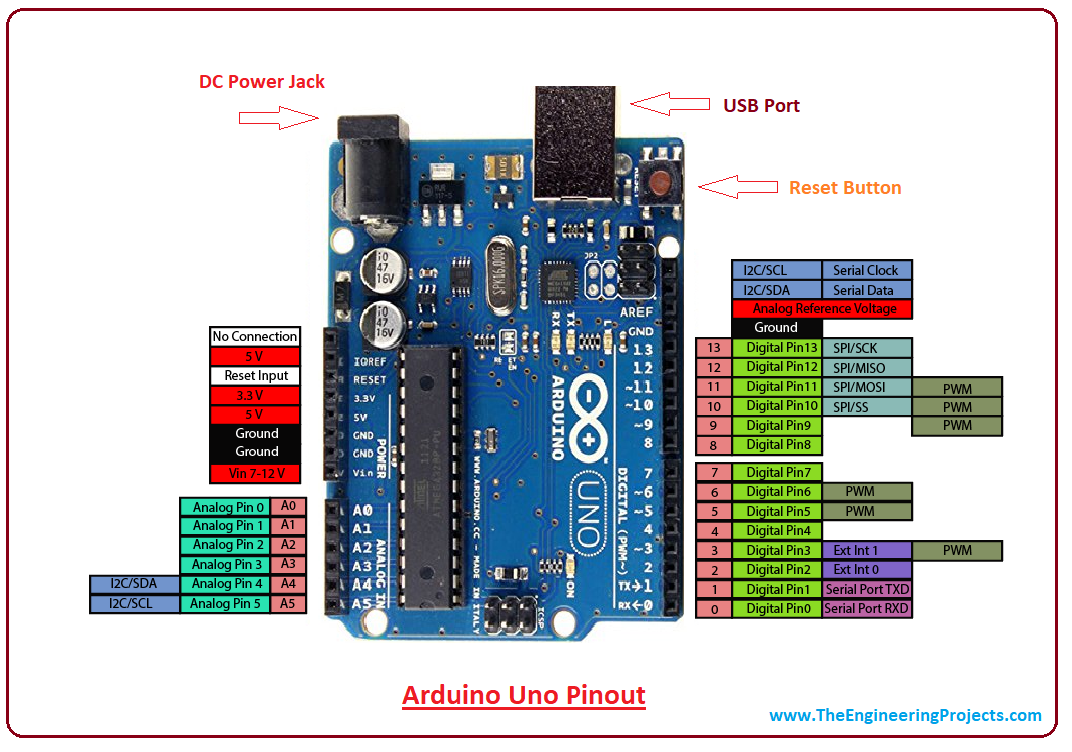
\includegraphics[width=\linewidth]{pinout.png}
                        \caption{\label{fig:pic}Arduino Uno Pinout}
                    \end{figure}
                \item \textbf{Pin Description}
                    \linebreak
                    \vspace{3mm}
                    \par \textbf{LED:} comes with build-in LED which is connected through pin 13.
                Providing HIGH value to the pin will turn it ON and LOW will turn it OFF. \\
                    \vspace{2mm}
                    \par \textbf{Vin:} input voltage provided to the Arduino Uno board. It's
                different than 5V supplied through the USB port. This pin is used to supply voltage. 
                If a voltage is provided through power jack, it can be accessed through this pin. \\
                    \vspace{2mm} 
                    \par \textbf{5V:} comes with the ability to provide voltage regulation. 5V pin is 
                used to provide output regulated voltage. The board is powered up using the 3 ways: 
                USB, Vin pin of the board or DC power jack. \\
                    \vspace{2mm}
                    \par \textbf{GND:} ground pins. More than one ground pins are provided 
                on the board which can be used as per requirement.
                    \vspace{2mm}
                    \par \textbf{Reset:} this is incorporated on the board which resets the 
                program running on the board. Instead of physical reset on the board, IDE comes 
                with a feature of resetting the board through programming. \\
                    \vspace{2mm}
                    \par \textbf{IOREF:} this pin very useful for providing voltage reference to 
                the board. A shield is used to read the voltage across this pin which then select 
                the proper power source. \\
                    \vspace{2mm}
                    \par \textbf{PWM:} is provided by 3,5,6,9,10; 11 pins. These pins are configured 
                to provided 8-bit output PWM. \\
                    \vspace{2mm}
                    \par \textbf{SPI:} It is known as Serial Peripheral Interface. 4 pins 10(SS), 11(MOSI), 
                12(MISO), 13(SCK) provide SPI coummunication with the help of SPI library. \\
                    \vspace{2mm}
                    \par \textbf{AREF:} called Analog Reference. This pin is used for providing a reference 
                voltage to the analog inputs. \\ 
                    \vspace{2mm}
                    \par \textbf{TWI:} called Two-tire Interface. TWI communication is accessed through 
                Wire Library. A4 and A5 pins are used for this purpose. \\
                    \vspace{2mm}
                    \par \textbf{Serial Communication:} is carried out through 2 pins call pin 0(Rx) and 
                pin 1(Tx). Rx pin is used to receive data while Tx pin is used to transmit data. \\
                    \vspace{2mm}
                    \par \textbf{External Interrupts:} Pin 2 and 3 are used for providing external interrupts. 
                An interrupt is called by providing LOW or changing value.
                \item \textbf{Communication and Programming} 
                    \linebreak
                    \vspace{3mm}
                    \par Arduino Uno comes with an ability of interfacing with other Arduino boards, 
                microcontrollers and computer. The ATMega328 placed on board provides serial communication 
                using pins like Rx and Tx. \\ 
                    \vspace{2mm}
                    \par Arduino Uno is programmed using Arduino Software which is a cross-platform application 
                call IDE(Intergrated Development Environment) written in Java. The AVR microcontroller ATMega328 
                laid out on the base comes with built-in bootloader that sets you free from using a separate 
                burner to upload the program on the board.
                \item \textbf{Application}
                    \linebreak
                    \vspace{3mm}
                    \par Arduino Uno comes with a wide range of Applications. A larger number of people 
                are using Arduino boards for developing sensors and instruments that are used in scientific 
                research. Following are some main applications of the board: \\
                    \vspace{2mm}
                    \par \guillemotright Embedded System \\
                    \par \guillemotright Security and Defense System \\
                    \par \guillemotright Digital Electronics and Robotics \\
                    \par \guillemotright Parking Lot Counter \\
                    \par \guillemotright Weighing Machines \\
                    \par \guillemotright Traffic Light Count Down Timer \\
                    \par \guillemotright Medical Instrument \\
                    \par \guillemotright Emergency Light for Railways \\
                    \par \guillemotright Home Automation \\ 
                    \par \guillemotright Industrial Automation \\
                    \vspace{2mm}
                    \par There are a lot of other microcontrollers available in the market that are 
                more powerful and cheap as compared to Arduino board. \\
                    \vspace{2mm}
                    \par Actually, Arduino comes with a big community that is developing and sharing the 
                knowledge with a wide range of audience. Quick support is available pertaining to technical 
                aspects of any electronic project.
            \end{enumerate}
        \subsubsection{\Large{Servo Motor}}
            \begin{enumerate}
                \item \textbf{Introduction}
                    \vspace{3mm}
                    \par Servo Motors(or servos) are self-contained electric devices that rotate or push 
                parts of machine with great precision. Servos are found in many places, from toys to home 
                electronics to cars and airplanes. If you have a radio-controlled model car, airplanes, 
                or helicopter, you are using at least a few servos. By rotating a shaft connected to the 
                engine throttle, a servo regulates the speed of a fuel-powered car or aircraft. \\
                    \vspace{2mm}
                    \par Servo also appear behind the scene in devices we use every day. Electronic device 
                such as DVD players use servos to extend or retract the disc trays.
                    \begin{figure}[ht]
                        \centering
                        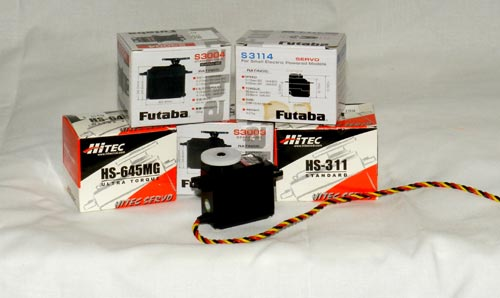
\includegraphics[width=0.6\linewidth]{Servo.jpg}
                        \caption{\label{fig:pic}Assortment of Servos}
                    \end{figure}
                \item \textbf{How does a servo work?}
                    \vspace{3mm}
                    \par The simple of a servo among the features that make them so reliable. 
                The heart of a servo is a small direct current (DC) motor, similar to what you 
                might find in an cheap toy. These motors run on electricity from a battery and spin 
                at high RPM(Rotations per minute) but put out very low \textbf{torque}(a twisting force 
                used to do work you apply torque when you open a bottle).
                    \begin{figure}[ht]
                        \centering
                        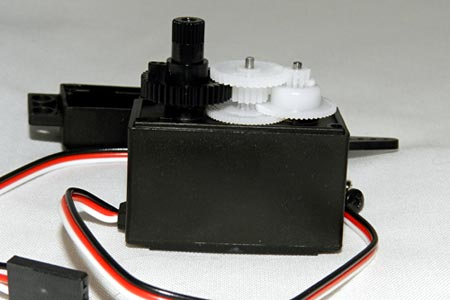
\includegraphics[width=0.6\linewidth]{Servo1.jpg}
                        \caption{\label{fig:pic}The Gears in a Typical Standard-size servo}
                    \end{figure}
                    \newpage
                    \par In high-power servo, the plastic gears are replaced by metal ones for strength. 
                    The motor is usually more powerful than in a low-power servo and the overall output torque 
                    can be as much as 20 times higher than a cheaper plastic one. Better quality is more 
                    expensive, and high-output servos can cost two or three times as much as standard ones.
                    \begin{figure}[ht]
                        \centering
                        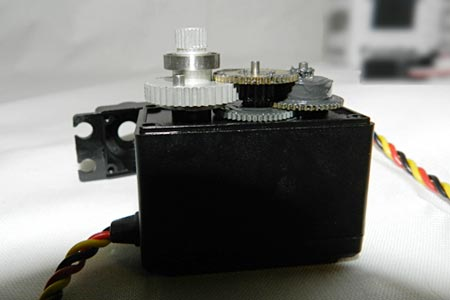
\includegraphics[width=0.6\linewidth]{Servo2.jpg}
                        \caption{\label{fig:pic}The gears in a Typical High-power servo}
                    \end{figure} 
                    \vspace{2mm}
                    \par With a small DC motor, you apply power from a battery, and the motor spins. 
                Unlike a simple DC motor, however, a servo's spinning motor shaft is slowed way down with 
                gears. A positional sensor on the final gear is connected to a small circuit board. The 
                sensor tells this circuit board how far the servo output shaft has rotated. The electronic 
                input signal from the computer or the radio in a remote-controlled vehicle also feeds into 
                that circuit board. The electronics on the circuit board decode the signals to determine 
                how far the user wants the servo to rotate. Then compares the desired position to the 
                actual position and decides which direction to rotate the shaft so it gets to the desired 
                position.
                    \begin{figure}[ht]
                        \centering
                        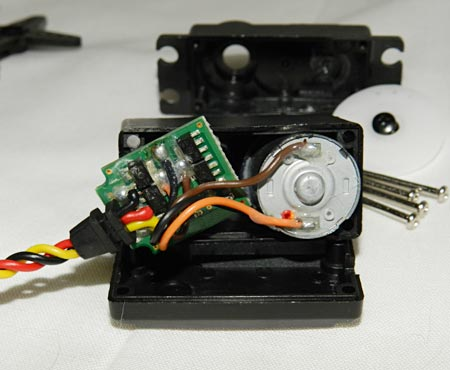
\includegraphics[width=0.4\linewidth]{Servo3.jpg}
                        \caption{\label{fig:pic}The circuit board and DC motor in a high-power servo}
                    \end{figure}
                \item \textbf{Types of servo motors}
                    \vspace{3mm}
                    \par Servos come in many sizes and in 3 basic types: 
                    \begin{itemize}
                        \item \textbf{Positional rotation servo:} This is the most common type of servo 
                    motor. The output shaft rotates in about half of a circle, or 180 degrees. It has physical 
                    stops placed in the gear machanism to prevent turning beyond these limits to protect the 
                    rotational sensor. These common servos are found in radio-controlled cars, aircraft, toys, 
                    robots and many applications. 
                        \item \textbf{Continuous rotation servo:} This is quite similar to the common positional 
                    rotation servo motor, except it can turn in either direction indefinitely. The control 
                    signal, rather than setting the static position of the servo, is interpreted as the direction 
                    and speed of rotation. The range of possible commands causes the servo to rotate clockwise 
                    or counterclockwise as desired, at varying speed, depending on the command signal. You might 
                    use a servo of this type on a radar dish if you mounted one on a robot. Or you could use 
                    one as a drive motor on a mobile robot.
                        \item \textbf{Linear servo:} This is also like the positional rotation servo motor described 
                    above, but with additional gears(usually a \textbf{rack and pinion} mechanism) to change 
                    the output from circular to back-and-forth. These servos are not easy to find, but you can 
                    sometimes find them at hobby stores where they are used as actuators in larger model airplanes.
                    \end{itemize}
                \item \textbf{Selecting a servo motor}
                    \linebreak
                    \vspace{3mm}
                    \begin{figure}[ht]
                        \centering
                        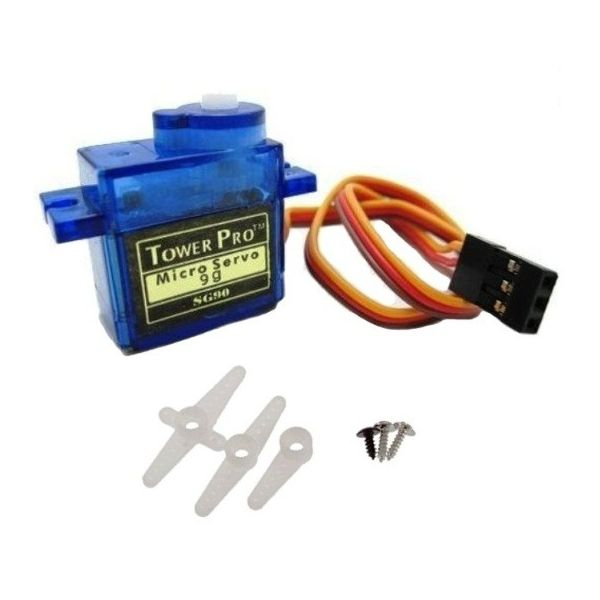
\includegraphics[width=0.3\linewidth]{sg90.jpg}
                        \caption{\label{fig:pic}Micro Servo 90}
                    \end{figure}
                    \newpage
                    Micro servo motor 90(SG90) is tiny and lightweight with high output power. This servo can 
                    rotate approximately 180 degrees (90 in each direction), it works just like the standard kinds 
                    but smaller. We can use any servo code, hardware or library to control this servo. It good for 
                    beginners who want to make stuff move without building a motor controller with feedback and gear 
                    box, especially since it will fit in small places.
                    \begin{figure}[ht]
                        \centering
                        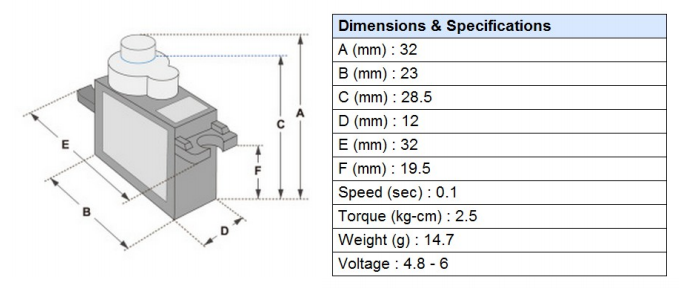
\includegraphics[width=\linewidth]{Capture.PNG}
                        \caption{\label{fig:pic}Section of SG90}
                    \end{figure}
                    \par \textbf{Block Diagram of SG90}
                    \begin{figure}[ht]
                        \centering
                        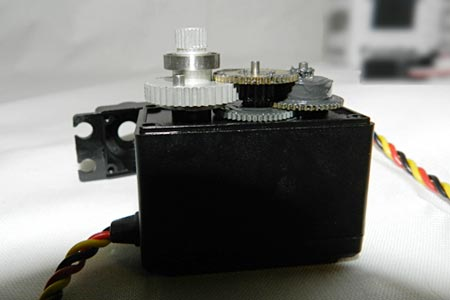
\includegraphics[width=0.6\linewidth]{Servo2.PNG}
                        \caption{\label{fig:pic}SG90 datasheet}
                    \end{figure}
                \item \textbf{Controlling a servo motor} 
                    \linebreak
                    \vspace{3mm}
                    \begin{figure}[ht]
                        \centering
                        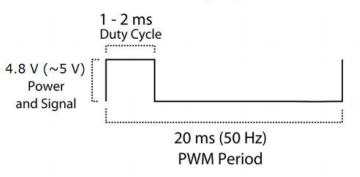
\includegraphics[width=0.4\linewidth]{servo3.PNG}
                        \caption{\label{fig:pic}PWN Period}
                    \end{figure}
                    \par Servo take commands from a series of pulse sent from the computer or radio. A pulse 
                is a transition from low voltage to high voltage which stays high for a short time, and then 
                returns to low. In battery devices such as servos, "low" is considered be ground or 0V 
                and "high" is the battery voltage. Servos tend to work in a range of 4.5 to 6 volts, so they 
                are extremely hobbyist computer-friendly.
            \end{enumerate}
        \subsubsection{\Large{HC-SR04 (Ultrasonic Sensor)}}
            \begin{enumerate}
                \item \textbf{Introduction}
                    \linebreak
                    \vspace{3mm}
                    \par An Ultrasonic Sensor is an electronic device that measures the distance 
                of target object by emitting ultrasonic sound waves, and converts the reflected sound 
                into an electrical signal. Ultrasonic waves travel faster than the speed of audible sound 
                (the sound that human can hear). \\
                    \vspace{2mm}
                    \par Transmitter and Receiver are two main parts of the sensor where former converts an 
                electrical signal to ultrasonic waves while later converts that ultrasonic signal back to 
                electrical signals. \\
                    \vspace{2mm}
                    \par Following table shows the main features of this ultrasonic sensor \\
                    \vspace{2mm}
                    \begin{table}[ht]
                        \centering
                        \begin{tabular}{ | l | l |}
                            \hline
                            \rowcolor{lightgray} Parameter & Value \\ \hline
                            Main Parts & Transmitter and Receiver \\ \hline
                            Operating Voltage & 5V \\ \hline
                            Operating Frequency & 4MHz \\ \hline
                            Detection Range & 2cm to 400cm \\ \hline
                            Measuring Angle & 30 degrees \\ \hline
                            Resolution & 3mm \\ \hline
                            Operating Current & < 15mA \\ \hline
                            Sensor Dimensions & 45mm x 20mm x 15mm \\ \hline
                        \end{tabular}
                        \caption{\label{tab:table}Feature of HC-SR04}
                    \end{table}
                    \vspace{2mm}
                    \par In order to calculate the distance between the sensor and the object, the sensor 
                measures the time it takes between the emission the sound by the transmitter to its contact with 
                the receiver. The formula for this calculation:
                    \begin{align*}
                        \centering
                        D = 1/2 * T * C
                    \end{align*}
                    \par Where: 
                    \begin{itemize}
                        \item D: the distance
                        \item T: the time
                        \item C: the speed of sound ~ 343 meter/second
                    \end{itemize} 
                \item HC-SR04 Pinout and Description
                    \linebreak
                    \vspace{3mm}
                    \par HC-SR04 contain 4 pins in total.
                    \begin{table}[ht]
                        \centering
                        \begin{tabular}{ | l | l | p{7cm} |}
                            \hline
                            \rowcolor{lightgray} No. & Pin name & Pin Description \\ \hline
                            1 & VCC & The power supply pin of the sensor that mainly operates at 5V DC \\ \hline
                            2 & TRIG Pin & It plays a vital role to initialize measurement for sending ultrasonic 
                            waves. It should be kept high for 10us for triggering the measurement \\ \hline
                            3 & ECHO Pin & This pin remains high for short period based on the time taken by the 
                            ultrasonic waves to bounce back to the receiving end \\ \hline
                            4 & Ground & This pin is connected to ground \\
                            \hline
                        \end{tabular}
                        \caption{\label{tab:table}Pinout of HC-SR04}
                    \end{table}
                    \par This figure below here is labelled these HC-SR04 Pinout for better visualization:
                    \begin{figure}[ht]
                        \centering
                        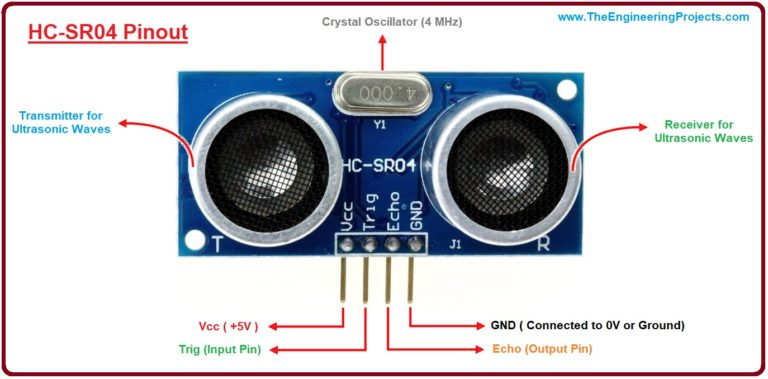
\includegraphics[width=\linewidth]{HC-SR04.jpg}
                        \caption{\label{fig:pic}HC-SR04 Pinout}
                    \end{figure}
                \item \textbf{How does it work?}
                    \begin{figure}[ht]
                        \centering
                        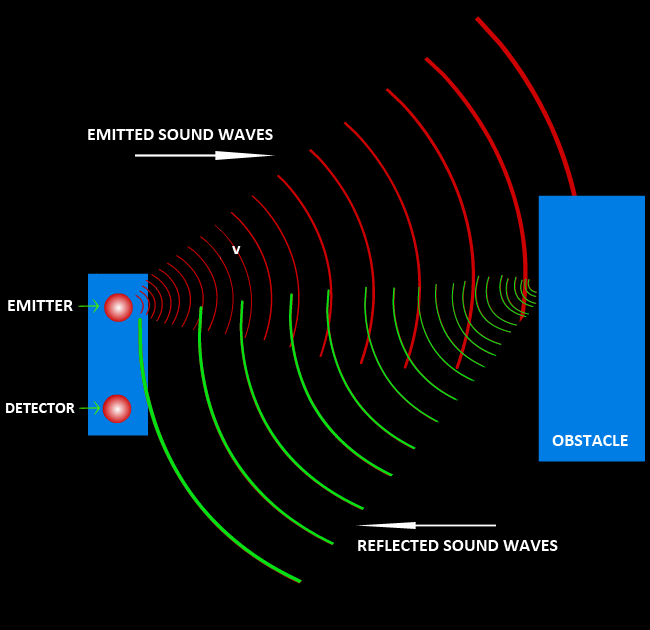
\includegraphics[width=0.4\linewidth]{ultrasonic_sensor.png}
                        \caption{\label{fig:pic}Ultrasonic sensor diagram}
                    \end{figure}
                    \linebreak
                    \par The \textbf{HC-SR04 Ultrasonic Sensor(US)} is an ultrasonic transducer that comes with 
                4 pin interface named as Vcc, Trigger, Echo, and Ground. It is very useful for accurate distance 
                measurement of the target object and mainly works on the sound waves. \\
                    \vspace{2mm}
                    \par As we connect the module to 5V and initialize the input pin, it starts transmitting 
                the sound waves which then travel through the air and hit the required object. These waves 
                hit and bounce back from the object and then collected by the receiver of the module. \\
                    \begin{figure}[ht]
                        \centering
                        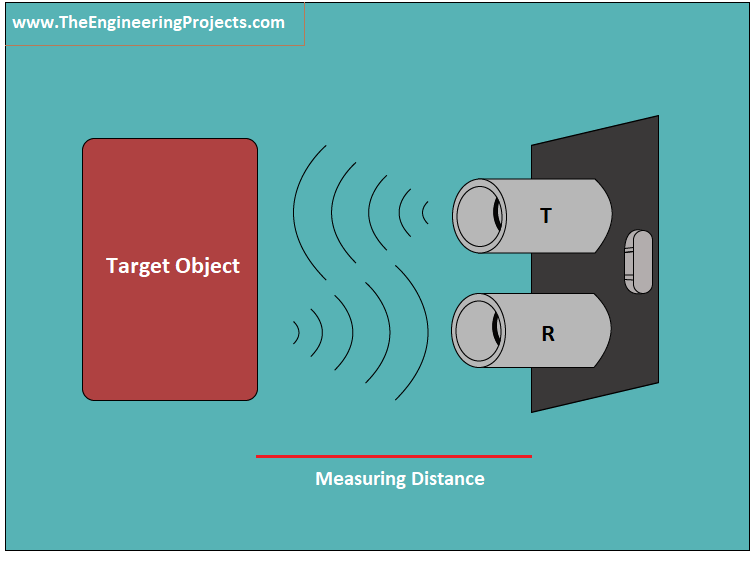
\includegraphics[width=0.6\linewidth]{ultrasonic.png}
                        \caption{\label{fig:pic}Principle of wave transmission}
                    \end{figure}
                    \par Distance is directly proportional to the time these waves require to come back at the 
                receiving end. The more the time taken, more the distance will be. \\
                    \vspace{2mm}
                    \par The waves will be generating if the Trig pin is kept high for 10$\mu$S. These waves 
                will travel at the speed of sound, creating 8 cycle sonic burst that will be collected in 
                the Echo pin. \\
                    \vspace{2mm}
                    \par The Echo pin remains turned on for the time these waves take to travel and bounce 
                back to the receiving end. This sensor is mainly incorporated with Arduino to measure the 
                required distance. \\
                    \vspace{2mm}
                    \par Following the formula is used to calculated the distance of the object. \\
                    \begin{align*}
                        \centering
                        S = (V*t)/2
                    \end{align*}
                    \par Where S is the required distance, V is the speed of sound and t is the time sound 
                waves takes to come back after hitting the object. We need to divide the value by 2 because 
                time will be double as the waves travel and bounce back from the initial point. Diving it by 
                2 will give the actual distance of the target object.
            \item \textbf{Application}
                    \linebreak
                    \vspace{3mm}
                    \par HC-SR04 comes with a widt range of applications mainly targeting distance and direction 
                measurement. Following are the major applications it can be used for: \\
                    \vspace{2mm}
                    \par \guillemotright Speed and direction measurement
                    \par \guillemotright Wireless charging
                    \par \guillemotright Humidifiers
                    \par \guillemotright Medical ultrasonography
                    \par \guillemotright Burglar alarms
                    \par \guillemotright Embedded system
                    \par \guillemotright Depth measurement
                    \par \guillemotright Non-destructive testing
            \end{enumerate}
        \subsubsection{\Large{LCD 16x02}}
            \begin{enumerate}
                \item \textbf{Introduction}
                    \begin{figure}[H]
                        \centering
                        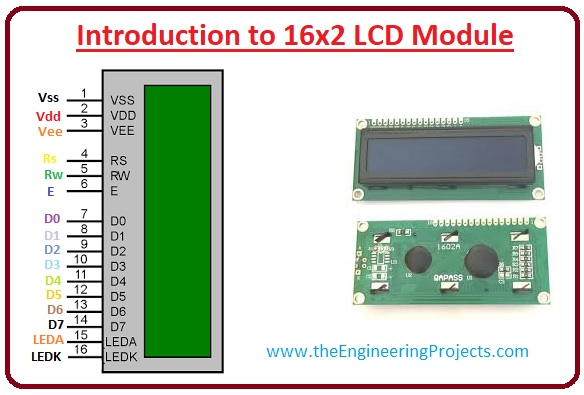
\includegraphics[width=0.4\linewidth]{LCD.jpg}
                        \caption{\label{fig:pic}LCD 16x2 Module}
                    \end{figure}
                    \par The liquid crystal display are normally used in different embedded projects due to 
                its low cost, easy access and flexibility to get programmed. \\
                    \vspace{2mm}
                    \par Almost each and every electronic device we daily see it like in your mobile, calculator 
                and some other devices. \\
                    \vspace{2mm}
                    \par There is a type of liquid display that has sixteen column and two rows so it is known 
                as 16 x 02 LCD modules. \\ 
                    \vspace{2mm}
                    \par LCD also available in different arrangements like (8x1), (10x2), (16x1), but the (16x2) 
                liquid crystal is normally used in embedded projects. \\
                    \vspace{2mm}
                    \par In this liquid crystal display, there are thirty-two characters and each of them consists 
                of 5x8 pixels. \\
                    \vspace{2mm}
                    \par So we can say that character consists of forty pixels or dots and total pixels in this 
                liquid crystal display can be fined as (32x40) or 1280 pixels. 
                \item \textbf{Block Diagram}
                    \begin{figure}[H]
                        \centering
                        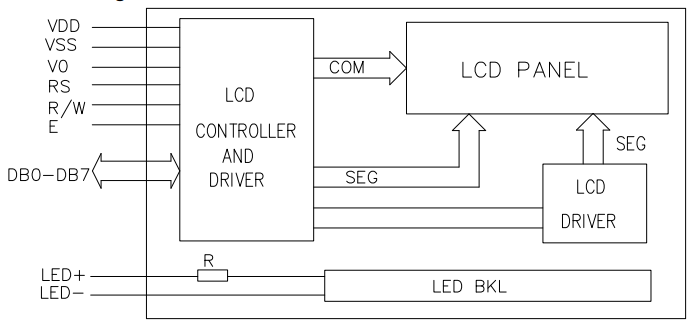
\includegraphics[width=\linewidth]{lcd diagram.PNG}
                        \caption{\label{fig:pic}Block Diagram of LCD}
                    \end{figure}
                \item \textbf{Pinout Description}
                    \linebreak
                    \par These are the main pinouts of 16x2 LCD that are described here with detailed: 
                    \begin{table}[H]
                        \centering
                        \begin{tabular}{ | p{1.2cm} | p{2.5cm} | p{7cm} | }
                            \hline
                            \rowcolor{lightgray} Pin No: & Pin name & Parameters \\ \hline
                            1 & Ground & This pin is used to connect the ground \\ \hline
                            2 & +5 Volt & At this pinout plus five volts are applied to on the LCD \\ \hline
                            3 & VE & This pin used to select the contract of the display \\ \hline
                            4 & Register Select & This pinout is used to MCU controller connected led to a 
                            shift from command to data mode \\ \hline
                            5 & Read and Write & It used for reading and wiring of data \\ \hline
                            6 & Enable & It linked with the MCU to toggle among zero and one \\ \hline
                            7 & Data PIN 0 & The pinouts from zero to seven are data pinouts and these are 
                            linked with the MCU for transmission of data. This liquid crystal module can also 
                            operate on the four-bit mode by working on o, 1, 2, and 3 pinouts and others are 
                            free \\ \hline
                            8 & Data PIN 1 & \\
                            \cline{1-3}
                            9 & Data PIN 2 & \\
                            \cline{1-3}
                            10 & Data PIN 3 & \\
                            \cline{1-3}
                            11 & Data PIN 4 & \\
                            \cline{1-3}
                            12 & Data PIN 5 & \\
                            \cline{1-3}
                            13 & Data PIN 6 & \\
                            \cline{1-3}
                            14 & Data PIN 7 & \\
                            \hline
                            15 & LED Positive & This pinout for turn backlight of led into positive \\ \hline
                            16 & Led Negative & Backlight liquid crystal display pinout negative terminal \\ 
                            \hline
                        \end{tabular}
                        \caption{\label{tab:table}Pinout of 16x2 LCD}
                    \end{table}
                \item \textbf{Command code for 16x2 LCD Module}
                    \begin{table}[H]
                        \centering
                        \begin{tabular}{| p{1cm} | p{1.5cm} | p{7cm} |}
                            \hline
                            Sr.NO & Hex Code & Parameters \\ \hline
                            1 & 1 & This command will remove data displaying on the screen of lcd \\ \hline
                            2 & 2 & It used to move back home \\ \hline
                            3 & 4 & It used to change location of a cursor to left side \\ \hline
                            4 & 6 & It changes the position of cursor to right side \\ \hline
                            5 & 5 & It used for shift display on right \\ \hline
                            6 & 7 & It used for Shift display one left \\ \hline
                            7 & 8 & It used to off the display and cursor will also off \\ \hline
                            8 & 0A & It used for both display off, a cursor on \\ \hline
                            9 & 0C & It used for display on, cursor also off \\ \hline
                            10 & 0E & By using this command we can on display, the cursor  will be blinking \\ \hline
                            11 & 0F & By this command Display will be on, the cursor also blinking \\ \hline
                            12 & 10 & It changes the location of a cursor to left \\ \hline
                            13 & 14 & It set cursor location to right \\ \hline
                            14 & 18 & It changes the location of the complete display to the left side \\ \hline
                            15 & 1C & It changes the location of the complete display to right side \\ \hline
                            16 & 80 & It used to move the cursor to the first line \\ \hline 
                            17 & C0 & It send the cursor to starting of the second line \\ \hline
                            18 & 38 & 2 lines and 5x7 matrix \\ 
                            \hline
                        \end{tabular}
                        \caption{\label{tab:table}Command code}
                    \end{table}
                \item \textbf{Features}
                    \par \guillemotright These are some features of 16x2 LCD module that are described with 
                the detailed \\
                    \par \guillemotright Its functioning voltages are from 4.7-5.3 volts \\ 
                    \par \guillemotright It uses one mA current for operation \\ 
                    \par \guillemotright In this liquid crystal display, we can work both alphabets and numbers \\
                    \par \guillemotright On this module, there are rows each has sixteen characters \\ 
                    \par \guillemotright Every character of this board has 5 x 8 or 40 pixels \\
                    \par \guillemotright It works on both four and eight bits mode \\ 
                    \par \guillemotright It display screen backlight is two colour green and blue \\
            \end{enumerate}
        \subsubsection{\Large{Buzzer}}
            \begin{enumerate}
                \item \textbf{General Introduction}
                    \begin{figure}[H]
                        \centering
                        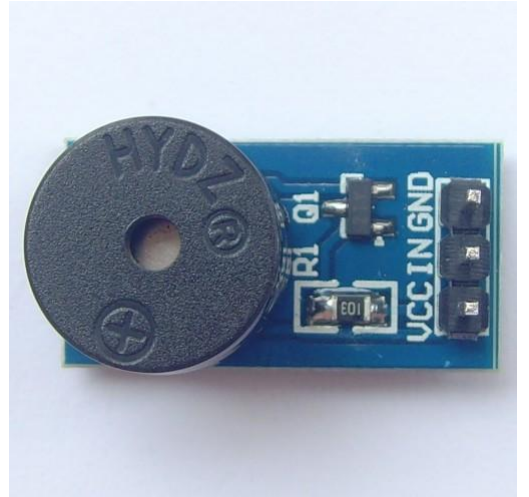
\includegraphics[width=0.4\linewidth]{buzzer.PNG}
                        \caption{\label{fig:pic}Buzzer}
                    \end{figure}
                    \par A buzzer or beeper is an audio signalling device, which maybe mechanical, electromechanical, 
                    or piezoelectric(piezo for short). Typical uses of buzzers and beepers include alarm devices, 
                    timers, and confirmation of user input such as a mouse click or keystroke. \\
                    \vspace{2mm}
                    \par Buzzer is an intergrated structure of electronic transducers, DC power supply, 
                    widely used in computers, printers, copiers, alarms, electronic toys,... Active buzzer 
                    5V rated power can be directly connected to a continuous sound, this section dedicated 
                    sensor expansion module and the board in combination, can complete a simple circuit design, 
                    to "plug and play".
                \item \textbf{Types of Buzzer}
                    \begin{itemize}
                        \item \textbf{Electromechanical:} Early devices were based on an electromechanical 
                        system identical to an electric bell without the metal gong. Similarly, a relay maybe 
                        connected to interrupt its own actuating current, causing the contacts to buzz. Often these 
                        units were anchored to a wall or ceiling to use it as a sounding board. The word "buzzer" 
                        comes from the rasping noise that electromechanical buzzers made.
                        \begin{figure}[H]
                            \centering
                            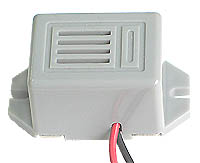
\includegraphics[width=0.3\linewidth]{buzzer1.jpg}
                            \caption{\label{fig:pic}Electromechanical Buzzer}
                        \end{figure}
                        \item \textbf{Mechanical:} A joy buzzer is an example of a purely mechanical buzzer and 
                        they require drivers. Other examples of them are doorbells.
                        \begin{figure}[H]
                            \centering
                            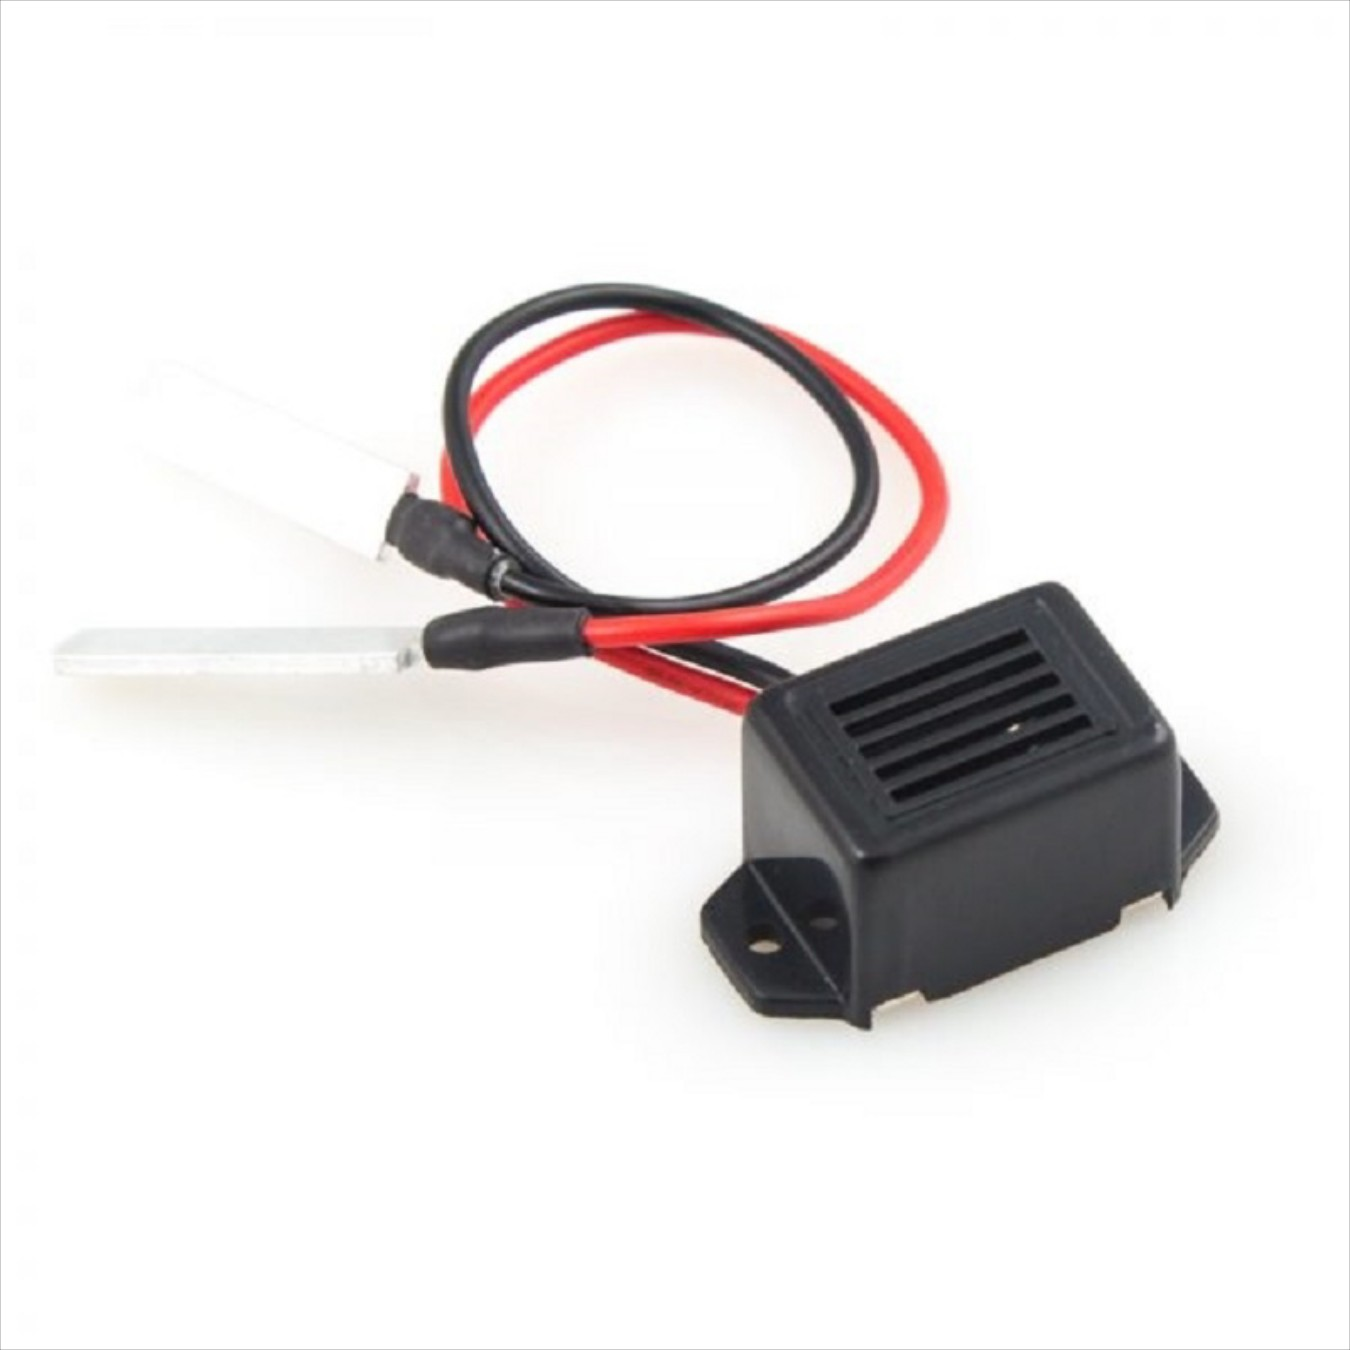
\includegraphics[width=0.4\linewidth]{buzzer2.jpg}
                            \caption{\label{fig:pic}Mechanical Buzzer}
                        \end{figure}
                        \item \textbf{Piezoelectric:} driven by an oscillating electronic circuit or other audio 
                        signal source, driven with a "piezoelectric audio amplifier". Sounds commonly used to indicate 
                        that a button has been pressed are a click, a ring or a beep. 
                        \begin{figure}[H]
                            \centering
                            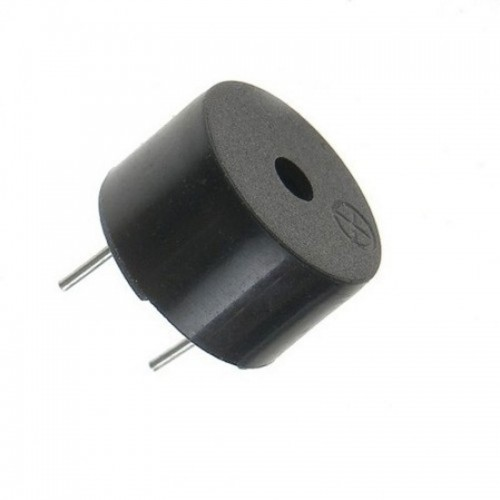
\includegraphics[width=0.3\linewidth]{buzzer.jpg}
                            \caption{\label{fig:pic}Piezoelectric Buzzer}
                        \end{figure}
                    \end{itemize}
                \item \textbf{Pin Configuration}
                    \begin{table}[H]
                        \centering
                        \begin{tabular}{|p{2cm}|l|p{7cm}|}
                            \hline
                            Pin Number & Pin Name & Description \\ \hline
                            1 & Positive & 	Identified by (+) symbol or longer terminal 
                            lead. Can be powered by 6V DC \\ \hline
                            2 & Negative & Identified by short terminal lead. Typically connected to 
                            the ground of the circuit \\ 
                            \hline
                        \end{tabular}
                    \end{table}
                    \begin{figure}[H]
                        \centering
                        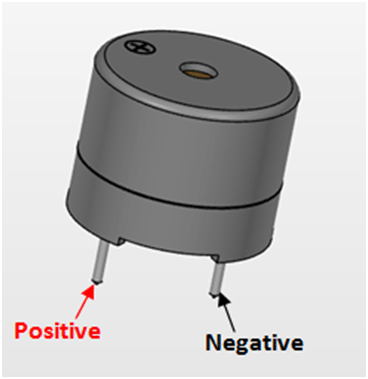
\includegraphics[width=0.4\linewidth]{buzzer-pinout.png}
                        \caption{\label{fig:pic}Buzzer Pinout}
                    \end{figure}
                \item \textbf{Features and Specifications}
                    \linebreak
                    \par \guillemotright Rated Voltage: 6V DC \\ 
                    \vspace{1mm}
                    \par \guillemotright Operating Voltage: 4-8V DC \\ 
                    \vspace{1mm}
                    \par \guillemotright Rated Current: <=30mA \\ 
                    \vspace{1mm}
                    \par \guillemotright Sound Output at 10cm: >=85dB \\
                    \vspace{1mm}
                    \par \guillemotright Sound Type: Continous Beep \\ 
                    \vspace{1mm}
                    \par \guillemotright Resonant Frequency: ~2300 Hz \\ 
                    \vspace{1mm}
                    \par \guillemotright Operating Temperature: $-25^{\circ}C$ to $80^{\circ}C$ \\
                    \vspace{1mm}
                    \par \guillemotright Storage Temperature: $-30^{\circ}C$ to $85^{\circ}C$ \\
                    \vspace{1mm}
                    \par \guillemotright Weight: 2g \\ 
                    \vspace{1mm}
                    \par \guillemotright Small and neat sealed package \\ 
                    \vspace{1mm}
                    \par \guillemotright Breadboard and Perf board friendly \\
                \item \textbf{Applications}
                    \begin{itemize}
                        \item Alarming Circuits, where the user has to be alarmed about something
                        \item Communication equipments
                        \item Automobile electronics
                        \item Portable equipments, due to its compact size
                    \end{itemize}
            \end{enumerate}

    \newpage
    \chapter{CONTENT AND RESULT}
    \renewcommand{\headrulewidth}{0.5pt}
    \renewcommand{\footrulewidth}{0.5pt}
    \thispagestyle{fancy}
    \fancyhf{}
    \fancyhead[L]{\textbf{CHAPTER 2}}
    \fancyhead[R]{\textbf{Radar Detector Module}}
    \raggedright
    \fancyfoot[R]{Page \thepage}
        \section{CONTENT}
            \subsection{{Block Diagram and Principles of Operation}}
                \subsubsection{\large{Block Diagram}}
                    \begin{figure}[H]
                        \centering
                        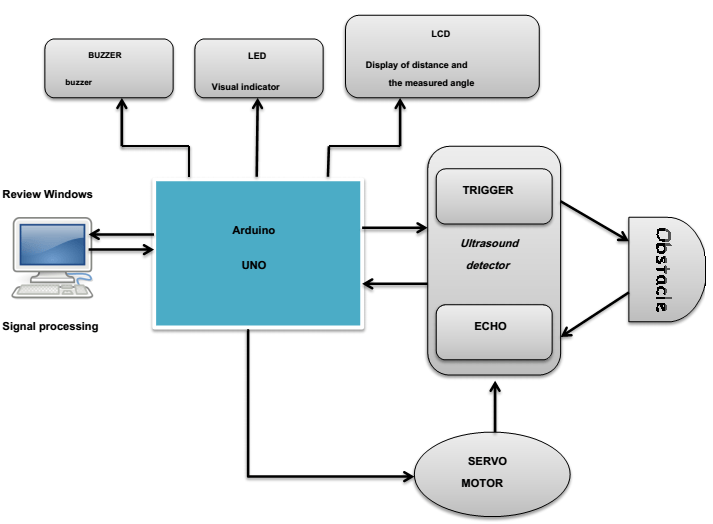
\includegraphics[width=0.8\linewidth]{diagram-project.png}
                        \caption{\label{fig:pic}Arduino Radar Using Ultrasonic Sensor}
                    \end{figure}
                    \par This diagram tell that Arduino is the interfaced with ultrasonic sensor. When the 
                    object is detected, the signal is given to the Arduino board which will below budget LED 
                    and LCD. That why mounted on ultrasonic sensors that will be rotating.
                \subsubsection{\large{Working of the project}}
                    \begin{figure}[H]
                        \centering
                        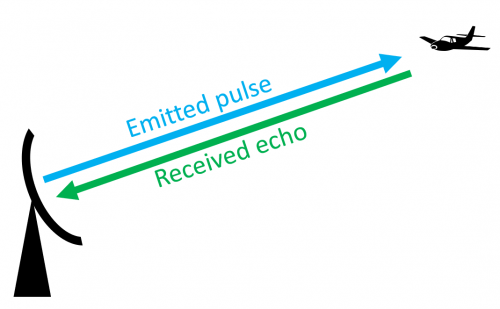
\includegraphics[width=0.6\linewidth]{500px-PSR_1.png}
                        \caption{\label{fig:pic}PSR principle of operation}
                    \end{figure}
                    Before we learn about how to this project working. We should find out how to conventional 
                    radar work. \\ 
                    \vspace{1mm}
                    \par In Aircraft Traffic Controlled, we have PSR (Primary Surveillance Radar), the antenna 
                    rotates (usually at 5-12rpm) emits a pulse of radiio wave. Upon reaching an aircraft 
                    (or other object) the wave is reflected and some of the energy is returned to the atenna.
                    \vspace{1mm}
                    \par The output data uses polar coordinate system - it provides range and bearing of the targets 
                    found in respect of the atenna position. Note that the range is the slant distance from 
                    the atenna and not the horizontal distance. \\ 
                    \vspace{1mm}
                    \par The range is determined by the time difference of the emitted and received pulse 
                    (the speed of propagation is the speed of the light) and the bearing is obtained from the 
                    atenna azimuth. The rotation speed of the atenna is usually between 5 and 12 rpm. \\
                    \vspace{1mm}
                    \par The antenna radiation pattern is a narrow beam when seen from above and, with some 
                    approximation, can be considered as a trapezium if seen from the side. \\
                    \vspace{1mm}
                    \par For the conventional radar, here is a summary of how radar works:
                        \begin{enumerate}
                            \item Magnetron generates high-frequency radio waves.
                            \item Duplexer switches magentron through the antenna.
                            \item Antenna acts as transmitter, sending narrow beam of radio waves through the air.
                            \item Radio waves hit enemy airplane and reflect back.
                            \item Atenna picks up reflected waves during a break between transmissions. Note that the same antenna 
                            acts as both transmitter and receiver, alternately sending out radio waves and receiving them.
                            \item Duplexer switches antenna through to receiver unit.
                            \item Computer in receiver unit processes reflected waves and draws them on TV screen.
                            \item Enemy plane shows up on TV radar display with any other nearby targets. 
                        \end{enumerate}
                        \begin{figure}[H]
                            \centering
                            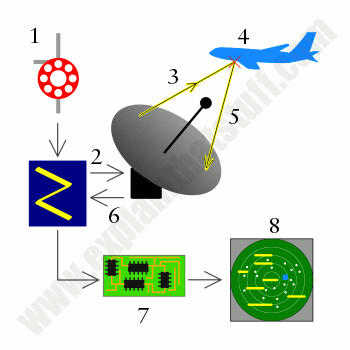
\includegraphics[width=0.8\linewidth]{radar-work.png}
                            \caption{\label{fig:pic}How a radar works}
                        \end{figure}
                    \par Now, in this project we will learn how this model working. \\
                    \vspace{3mm}
                    \Large{\textbf{FLOWCHART OF MODEL}}
                    \begin{figure}[H]
                        \centering
                        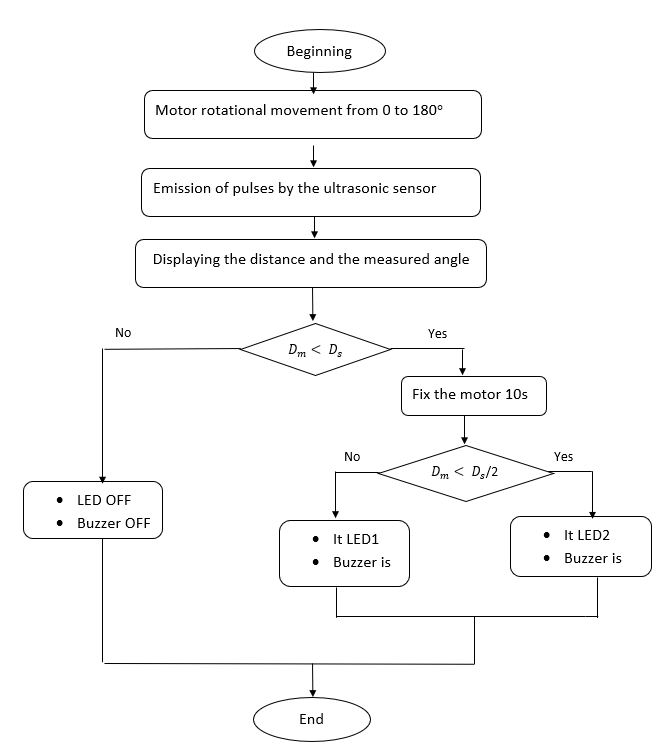
\includegraphics[width=\linewidth]{flowchart1.png}
                        \caption{\label{fig:pic}Flowchart}
                    \end{figure}
                    \large{
                        Arduino board sends a signal of 5V to TRIG pin of Ultrasonic Sensor HC-SR04 
                    which triggers the sensor. Then it procides rotational action at the servo motor mechanically 
                    fitted along with Ultrasonic sensor so that it can detec the moving objects and locate within 
                    180 degrees. \\ 
                    \vspace{1mm}
                    \par The Arduino sends a HIGH pulse width of (10 S) on the TRIGGER pin of the sensor to 
                    regenerate  a series of ultrasonic waves which propagate through the air, until it touches 
                    an obstacle and returns in the opposite direction towards the sensor pin ECHO. The sensor 
                    detecs the width of the pulse to calculate the distance. \\
                    \vspace{1mm}
                    \par The signal on ECHO pin of the sensor remains at the HIGH position during transmission, 
                    thereby measuring the duration of the round trip of ultrasound and thus determine the distance. \\
                    \vspace{1mm}
                    \par The LCD display displays the calculated distance and the angle of rotation. The buzzer 
                    is an additional component, it rings when there is a detection (Tone 1 and Tone 2) along 
                    with the LEDs. These both LEDs along with buzzer determine the field where the object is 
                    located (near or distant). \\}
        \section{CIRCUIT DIAGRAM AND RESULT}
            \subsection{\large{Circuit Diagram}}
                \begin{figure}[H]
                    \centering
                    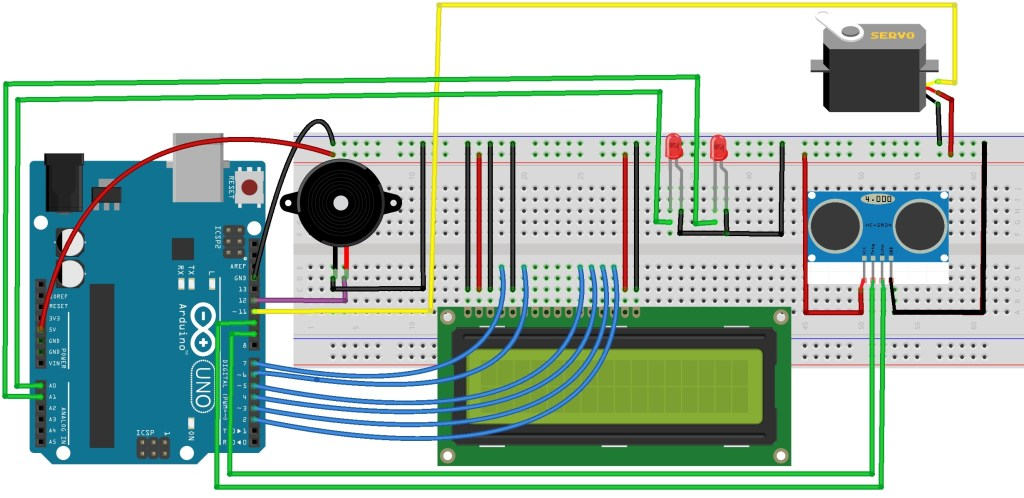
\includegraphics[width=\linewidth]{circuit.jpg}
                    \caption{\label{fig:pic}Circuit Diagram}
                \end{figure}
            \subsection{Result}

    \chapter{APPENDIX}
    \renewcommand{\headrulewidth}{0.5pt}
    \renewcommand{\footrulewidth}{0.5pt}
    \thispagestyle{fancy}
    \fancyhf{}
    \fancyhead[L]{\textbf{CHAPTER 3}}
    \fancyhead[R]{\textbf{Radar Detector Module}}
    \raggedright
    \fancyfoot[R]{Page \thepage}
        In this chapter, i'll present the code i have put in my project. \\
        \vspace{3mm}
        \par The code below here used to include the library. Libraries are files that you can 
        include in my code to use even more methods and functions. \\
        \vspace{2mm}
        \fbox{\begin{varwidth}{\dimexpr\textwidth-2\fboxsep-2\fboxrule\relax}
            \raggedright
            \# include <Servo.h> \\
            \# include <LiquidCrystal.h> \\
            \# include <Wire.h> \\
        \end{varwidth}}
        \vspace{3mm}
        \linebreak
        Next, we will create a variable "myServo" with datatypes is "Servo" and an LCD object 
        with parameters: (rs,enable,d4,d5,d6,d7). \\
        \vspace{2mm}
        \fbox{\begin{varwidth}{\dimexpr\textwidth-2\fboxsep-2\fboxrule\relax}
            \raggedright
            Servo myServo; \\
            LiquidCrystal lcd(7,6,5,4,3,2);
        \end{varwidth}}
        \vspace{3mm}
        \linebreak
        We will create some variables and asign each variable with 1 value. \\
        \vspace{2mm}
        \fbox{\begin{varwidth}{\dimexpr\textwidth-2\fboxsep-2\fboxrule\relax}
            \raggedright
            int pos = 0; // Original position of the servomotor \\
            const int trigPin = 9; \\
            const int echoPin = 10; \\
            const int moteur = 11; \\
            const int buzzer = 12; \\
            const int ledPin1 = 14; \\
            const int ledPin2 = 15; \\
            float distanceCm, DistanceSec,duration; \\
        \end{varwidth}}
        \vspace{3mm}
        \linebreak
        In setup() function is the code where we want to run one times as soon as program starts 
        running. In this function we'll set things like pinMode in it. \\
        \vspace{2mm}
        \fbox{\begin{varwidth}{\dimexpr\textwidth-2\fboxsep-2\fboxrule\relax}
            \raggedright
            void setup() \{ \\
                myServo.attach(moteur); // Attach the servo motor to pin 11 \\
                lcd.begin(16,2); // Initialize the Lcd interface with their Size \\
                pinMode(trigPin, OUTPUT); // Define the operation of these input/output pins. \\
                pinMode(echoPin, INPUT); \\
                pinMode(buzzer, OUTPUT); \\
                pinMode(ledPin1, OUTPUT); \\ 
                pinMode(ledPin2, OUTPUT); \\
                DistanceSec=20;\} \\ 
        \end{varwidth}}
        \newpage
        Next to these code is "void loop()" function which is uses as a part of its structure. 
        The code inside this function runs over and over as long as the Maker Board is turned on. \\
        \vspace{2mm} 
        Below here is the part 1. \\
        \vspace{2mm}
        \fbox{\begin{varwidth}{\dimexpr\textwidth-2\fboxsep-2\fboxrule\relax}
            \raggedright
            void loop() \{ \\
                for (pos = 0; pos <= 180; pos += 1) \{ // goes from 0 to 180 degrees\\
                // in steps of 1 degree\\
                myServo.write(pos); // Servo programming to get to the position (pos)\\
                digitalWrite(trigPin, LOW);\\
                delayMicroseconds(2);\\
                digitalWrite(trigPin, HIGH); // send a pulse of 10 microseconds\\
                delayMicroseconds(10);\\
                digitalWrite(trigPin, LOW);\\
                duration = pulseIn(echoPin, HIGH);\\
                distanceCm= duration*0.034/2;\\
                if (distanceCm <= DistanceSec)\{\\
                    if(distanceCm <= DistanceSec/2)\\
                    \{\\
                        tone(buzzer, 10); // Send 1KHz sound signal...\\
                        digitalWrite(ledPin1, LOW);\\
                        digitalWrite(ledPin2, HIGH);\\
                        delay(700);\\
                        noTone(buzzer); // Stop sound...\\
                        lcd.setCursor(0,0); // Position the cursor at 0.0\\
                        lcd.print("Distance: "); // Print "Distance" to LCD\\
                        lcd.print(distanceCm); // Print the distance to LCD\\
                        lcd.print(" cm "); // Print the unit sur LCD\\
                        delay(10);\\
                        lcd.setCursor(0,1);\\
                        lcd.print("Angle : ");\\
                        lcd.print(pos);\\
                        lcd.print(" deg ");\\
                        delay(2000);\\
                \}\\
        \end{varwidth}}
        \vspace{2mm}
        \linebreak
        Next, we have part 2 of this function. This for loop used for set the rotation of servo 
        to go 180$^{\circ}$.\\
        \vspace{2mm}
        \fbox{\begin{varwidth}{\dimexpr\textwidth-2\fboxsep-2\fboxrule\relax}
            \raggedright
            else\{\\
                digitalWrite(buzzer, HIGH);\\
                digitalWrite(ledPin2, LOW);\\
                digitalWrite(ledPin1, HIGH);\\
                delay(100);\\
                digitalWrite(buzzer, LOW);\\
                lcd.setCursor(0,0); // Position the cursor at 0.0\\
                lcd.print("Distance: "); // Print "Distance" sur LCD\\
                lcd.print(distanceCm); // Print the distance to LCD\\
                lcd.print(" cm "); // Print the unit to LCD\\
                delay(10);\\
                lcd.setCursor(0,1);\\
                lcd.print("Angle : ");\\
                lcd.print(pos);\\
                lcd.print(" deg ");\\
                delay(2000);\\
            \} \\
        \}\\
        else\{\\
            digitalWrite(buzzer, LOW);\\
            digitalWrite(ledPin1, LOW);\\
            digitalWrite(ledPin2, LOW);\\
        \}\\
        lcd.setCursor(0,0); // Position the cursor at 0.0\\
        lcd.print("Distance: "); // Print "Distance" sur LCD\\
        lcd.print(distanceCm); // Print the distance to LCD\\
        lcd.print(" cm "); // Printe the unit to LCD\\
        delay(10); \\
        lcd.setCursor(0,1); \\
        lcd.print("Angle : "); \\
        lcd.print(pos); \\
        lcd.print(" deg "); \\
        delay(80); // wait 100ms for the servo to find its position \\
        \} \\
        \end{varwidth}}
        \vspace{2mm}
        \linebreak
        Part 3 is the for loop to set the rotation cycle of servo motor. In this part, the for 
        loop will be identical to the for loop i mentioned above in part 2. This for loop make 
        a servo go back 180$^{\circ}$. 

    \chapter{CONCLUSIONS AND RECOMMENDATIONS}
    \renewcommand{\headrulewidth}{0.5pt}
    \renewcommand{\footrulewidth}{0.5pt}
    \thispagestyle{fancy}
    \fancyhf{}
    \fancyhead[L]{\textbf{CHAPTER 4}}
    \fancyhead[R]{\textbf{Radar Detector Module}}
    \raggedright
    \fancyfoot[R]{Page \thepage}
        
\end{document}